\documentclass[../rapport_MVEX01-11-05]{subfiles}
\begin{document}

\section{Klassificering av gester med hjälp av \knn}
Den största andelen korrekt klassificerade gester vi lyckades uppnå
med samtliga gester tillåtna var 91.9\,\%, både med forward selection
och backward elimination. Antalet aktiverade
egenskaper var 10 då forward selection-algoritmen användes och 7 med
backward selection, och antalet närmsta grannar i \knn-metoden var 7. Egenskaperna som
användes är listade i
tabell~\vref{tab:bestfeatsfwd}. Figur~\vref{fig:knn-optimering} visar mer
exakt hur andelen korrekta
klassficeringar beror på antalet aktiverade egenskaper och värdet på $k$.

\begin{figure}[tbp]
  \centering
  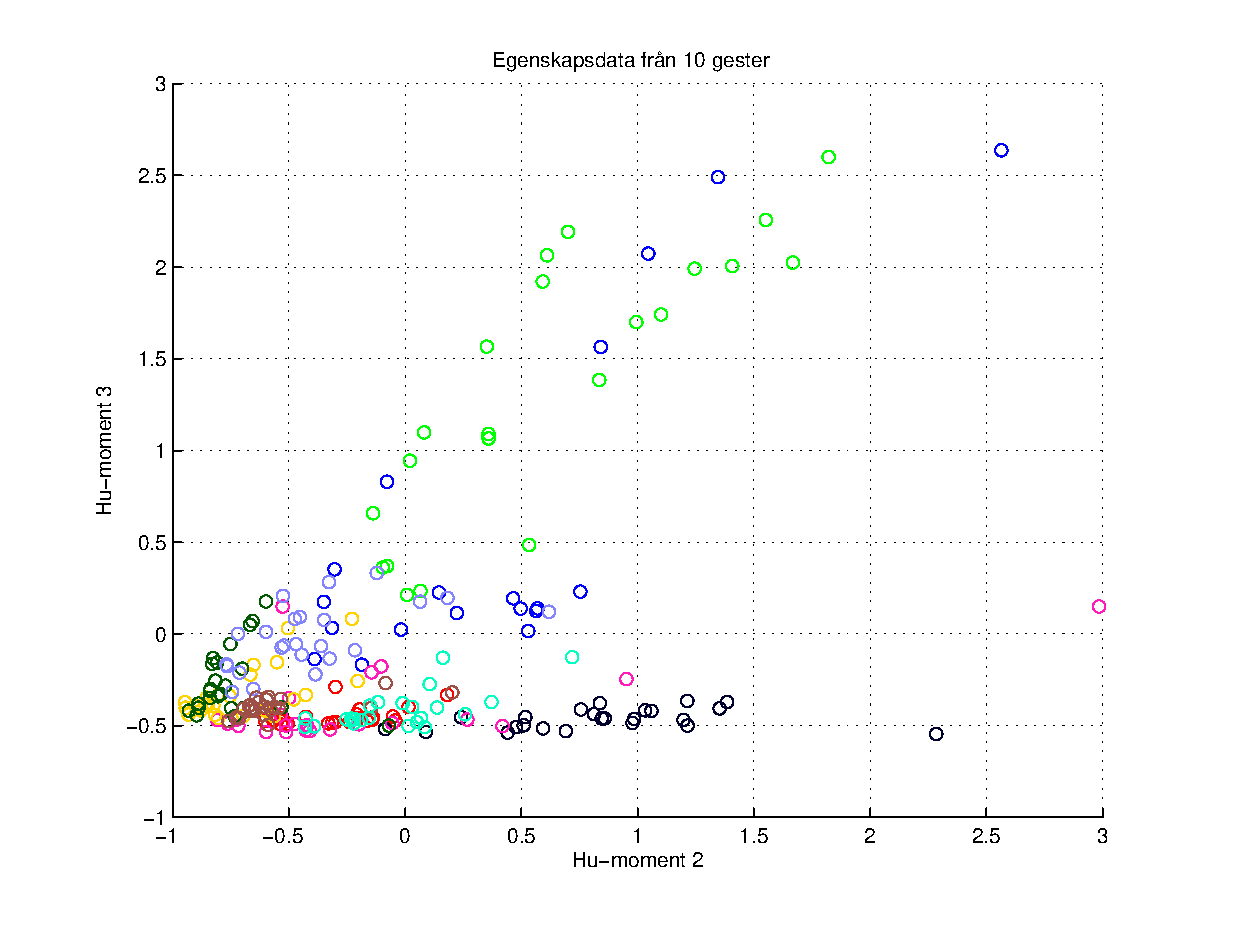
\includegraphics[width=\textwidth,trim=2cm 0.5cm 2cm 0,clip=true]{bilder/feats-10+11}
  \caption{Träningsmängden för ett urval av sex gester plottade mot de två
	starkaste egenskaperna. Notera hur de flesta är tydligt samlade, men att
	de även överlappar varandra.}
  \label{fig:feats1011}
\end{figure}

\begin{figure}[tbp]
    \begin{center}
        \subfloat[Forward selection]{
        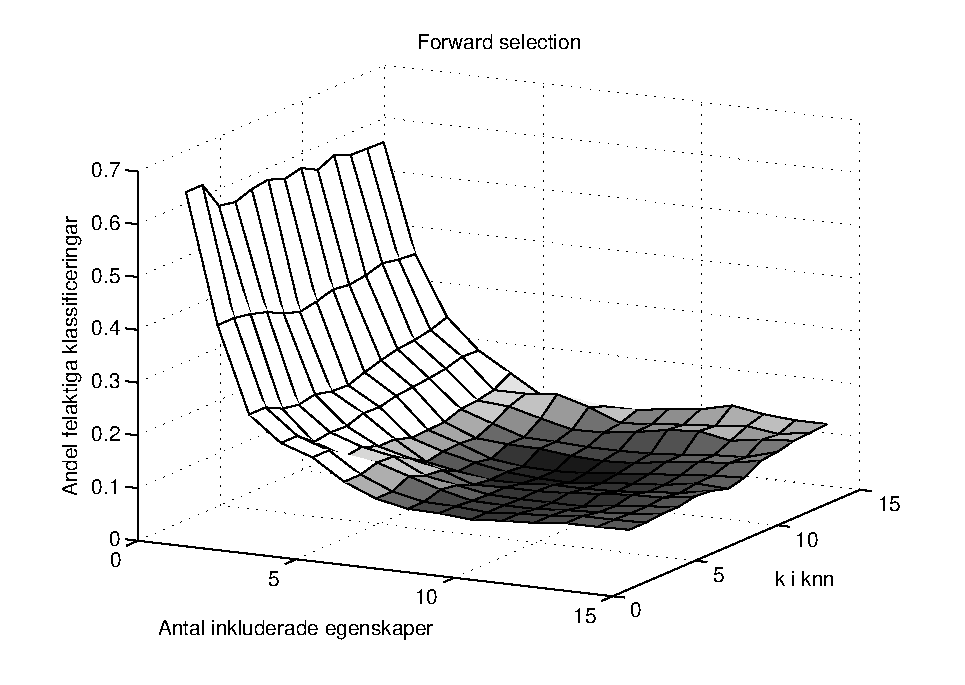
\includegraphics[width=0.5\columnwidth,clip=true]{bilder/fwd_sel.eps}
        \label{fig:fwd_sel}}
				%\\\medskip
        \subfloat[Backward selection]{
        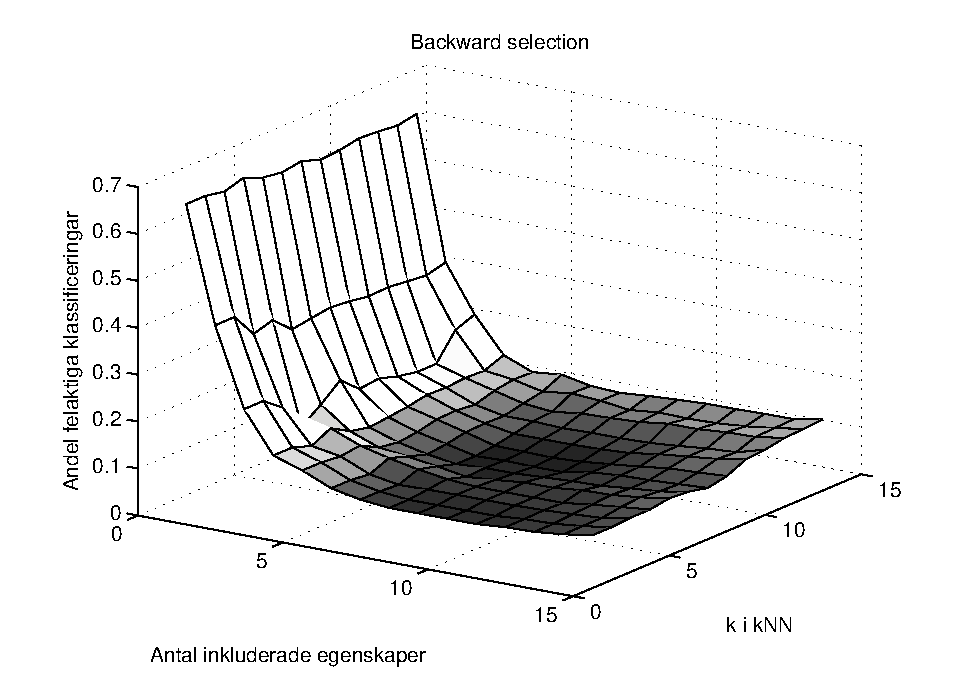
\includegraphics[width=0.5\columnwidth,clip=true]{bilder/bwd_sel.eps}
        \label{fig:bwd_sel}}
    \end{center}
    \caption{Optimering av \knn-metoden med avseende på inkluderade egenskaper
och värden på $k$. Med forward selection-algoritmen fås ett minimum då
$k=7$ och 10 egenskaper inkluderades. Med backward elimination fås
samma andel korrekta klassificeringar som minimum med $k=7$ och 7 inkluderade egenskaper.}
    \label{fig:knn-optimering}
\end{figure}

Det framgår tydligt att antalet aktiverade egenskaper har stor
inverkan på resultatet då man använder sig av färre än
fem. Därefter planar andelen ut för att återigen stiga då
fler än 10 egenskaper används. Andelen felklassificeringar
minskar också i takt med att $k$ ökar från 1 till 7, för att sedan
öka då värdet ökar från 7 till 13. Med valet av egenskaper och $k$ från
optimeringen med forward selection presterade metoden enligt
tabell~\vref{tab:tolkningsmatris} och tabell~\vref{tab:prestanda}.

\notes{(Inkludera resultat där problemgester är borttagna?)}

\begin{table}[tbp]
	\centering
	\caption{Felklassificeringar av statiska gester. Priori-fel
	betecknar sådana fel då gesten varit känd men identifierats
	som något annat; posteriori-fel betecknar sådana fel då
	identifikationen är känd men felaktig. \notes{Relatera till
	värden i tabell~\vref{tab:tolkningsmatris}}}
	\smallskip
	\label{tab:prestanda}
	\begin{tabular}{c c c}
		\toprule 
		Försöksgest & A Priori-fel & A Posteriori-fel \\
		\midrule 
		A & & \\
		B & & \\
		C & & \\
		D & & \\
		E & & \\
		Sten & & \\
		Sax & & \\
		Påse & & \\
		Spock & & \\
		Seger & & \\
		\bottomrule 
	\end{tabular}
\end{table}

\begin{table}[tbp]
	  \centering
		\caption{Vid försök misstolkas en del gester betydligt oftare än
		andra. Notera att raderna inte adderar till 100 eftersom värdena är
		avrundade.}
		\label{tab:tolkningsmatris}
    \includegraphics[trim=2cm 16cm 8cm 2.5cm,clip=true,width=8cm]{bilder/tolkningsmatris.pdf}
\end{table}

\begin{table}[tb]
	\centering
	\caption{De tio bästa egenskaperna med forward selection.}
	
	\label{tab:bestfeatsfwd}
	\begin{tabular}{ll}
		\toprule
		Ranking & Egenskap \\
		\midrule
		1 & Hu-moment 3 \\
		2 & Hu-moment 2 \\
		3 & Tyngdpunktsläge, $y$-led \\
		4 & Fyrkantighet \\
		5 & Soliditet \\
		6 & Excentricitet \\
		7 & Konvexitet \\
		8 & Hu-moment 1 \\
		9 & Utsträckning \\
		10 & Hu-moment 7 \\
		\bottomrule
	\end{tabular}
\end{table}

\begin{table}[tb]
	\centering
    \caption{De sju bästa egenskaperna med backward elimination.}
	
	\label{tab:bestfeatsbwd}
	\begin{tabular}{ll}
		\toprule
		Ranking & Egenskap \\
		\midrule
                1 & Fyrkantighet \\
                2 & Tyngdpunktsläge, $y$-led \\
                3 & Hu-moment 1\\
                4 & Soliditet\\
                5 & Konvexitet \\
                6 & Utsträckning \\
                7 & Hu-moment 3 \\
		\bottomrule
	\end{tabular}
\end{table}

\subsection{Egenskaper}\label{sec:resultat_features}

Egenskaperna vi använt har visat sig vara mycket bra, upp till en viss gräns.
I tabell~\vref{tab:bestfeatsfwd} syns de tio egenskaper som inkluderades
med forward selection. Av dessa kan man ta bort tre, excentricitet,
Hu-moment 2 och Hu-moment 7,
med samma resultat, enligt resultat från backward
elimination-algoritmen. De sju egenskaper som lämnas kvar med
backward elimination listas i tabell~\vref{tab:bestfeatsbwd}, i
ordning efter hur länge de är kvar i körningen.

Rankingen för samtliga egenskaper med de respektive metoderna finns i appendix
\ref{sec:egenskapsresultat}.

Ett urval av sex gester visar i
figur~\vref{fig:feats1011} hur de två bästa egenskaperna tydligt samlar varje
gest i ett relativt litet område, vilket gör att avstånden i \knn-metoden 
blir mindre, och att det därför blir enklare att sätta en tröskel för att
kunna klassificera ickegester. Det ska dock även noteras att egenskaperna 
överlappar varandra för vissa gester vilket sannolikt minskar träffsäkerheten.

\end{document}
